
Per controllo di assetto intendiamo un blocco funzionale dell'architettura di
controllo responsabile di:
\begin{itemize}
  \item Orientamento del veicolo;
  \item Stabilizzazione del veicolo intorno ad un assetto di riferimento in
  presenza di coppie perturbanti;
\end{itemize}
Tali obiettivi vengono raggiunti dotando il veicolo di sensori di assetto e di
attuatori correttamente dimensionati.
Fondamentale per effettuare un controllo di assetto è lo studio delle proprietà
del veicolo quali:
\begin{itemize}
  \item Posizione del Centro Di Massa
  \item Massa
  \item Momento di inerzia
  \item Variazioni dei parametri precedenti dovute a
  \begin{itemize}
    \item Consumo di propellente
    \item Deployment e orientamento di pannelli solari
    \item Deployment e orientamento di antenne
  \end{itemize}
\end{itemize}

\'{E} possibile suddividere il controllo di assetto in diverse fasi:
\begin{description}
\item[Orbit insertion:] Modalità impiegata durante l'immissione in orbita da
parte dell'ultimo stadio del lanciatore
\item[Acquisition:] Modalità impiegata durante la prima acquisizione
dell'assetto, consiste nel \emph{damping} della velocità angolare imposta
dall'ultimo stadio del lanciatore e successivamente nell'acquisizione di un
assetto tale a soddisfare le caratteristiche termiche ed elettriche necessarie
all'autonomia del satellite
\item[Normal:] Modalità impiegata durante le normali missioni consiste nel test
di tutti gli strumenti e nelle manovre orbitali
\item[Science:] Modalità impiegata qualora il satellite avesse dei requisiti
stringenti di precisione a causa di particolari strumenti impiegati in missioni
di ricerca
\item[Contingency o Safe:] Modalità impiegata in caso di \emph{failures} per
mettere in sicurezza il satellite.
\end{description}
%###
\subsection{Architettura e obbiettivi}
Obiettivo del controllo orbitale drag-free è la cancellazione delle forze non
gravitazionali agenti sul satellite per rendere il moto del centro di massa del
satellite dovuto con accettabile approssimazione esclusivamente alle forze
gravitazionali. L'accelerazione del centro di massa del satellite è descritta
dalle seguenti relazioni (tutte le coordinate sono espresse nel riferimento
corpo):

\begin{equation}
\components{\dot{v}}(t) = \components{g}(\components{r}(t))+
\frac{R_b(\quat{q})(-\components{F_d}(t)+\components{F_t}(t))}{m},
\components{v(0)=v_	0}
\end{equation}
dove $\components{F_d}$ sono le forze non gravitazionali (principalmente
aerodinamiche in orbita bassa) e $\components{F_t}$ sono le forze di comando
dovute ai propulsori.

Il controllo drag-free è soddisfatto quando la seguente relazione è soddisfatta:

\begin{equation}
\components{a}(t) = \frac{(- \components{F_d}(t) + \components{F_t}(t))}{m}=0
\end{equation}
ovvero l'accelerazione residua dovuta a componenti non gravitazionali
($\components{a}$) è nulla.

L'architettura prescelta per la compensazione delle forze suddette è basata 
sull' embedded model, essa è rappresentata in figura \ref{fig:orbit_control} e
corrisponde alle seguenti equazioni (introdurremo l'equazione del comando
nella prossima sezione):

\begin{IEEEeqnarray}{rCl}
	x(i+1)&=&(1-\beta)x(i) + \beta(d(i)+w_0(i)+u(i))\nonumber\\
	y(i)&=&x(i)+e(i) = y_m(i)+ e(i)
\end{IEEEeqnarray}
Di seguito una descrizione delle componenti dell'architettura di controllo e
dei parametri delle equazioni:
\begin{description}
\item[Dinamica Controllabile:] Descrive la dinamica tra comando e misura, deve
catturare le dinamiche ad alta frequenza il più vicino possibile alla più alta
componente in frequenza dei disturbi da cancellare.
\item[Dinamica del Disturbo:] Dinamica rappresentante il disturbo e modellata su
base statistica, comprende principalmente le forze aerodinamiche modellate sulla
base della loro densità spettrale
\item[Beta ($\beta$):] Compreso tra zero e 1 serve a modellare il ritardo
ingresso uscita tra l'applicazione del comando e la misura
\item[Disturbi prevedibili ($x_{d1} = a_{d} +d_{a}$):] Rappresentano la somma di
accelerazioni non gravitazionali ($a_{d}$) e disturbi sull'accelerometro
($d_{a}$, bias e/o drift)
\item[Disturbo dei propulsori ($w_0$):] Rumore bianco rappresentante la
caratteristica del rumore prodotto dai propulsori
\item[Comando ($u$):] Accelerazione comandata $\frac{\components{F_t}}{m}$
\item[Uscita del sistema ($y$):] \'{E} la misura rilevata dall'accelerometro
corrotta da eventuali disturbi e da cui sottraendo l'uscita del modello ($y_m$)
è possibile ricavare l'errore di modello utilizzato per aggiornare lo stato del
modello
\end{description} 

\begin{figure}
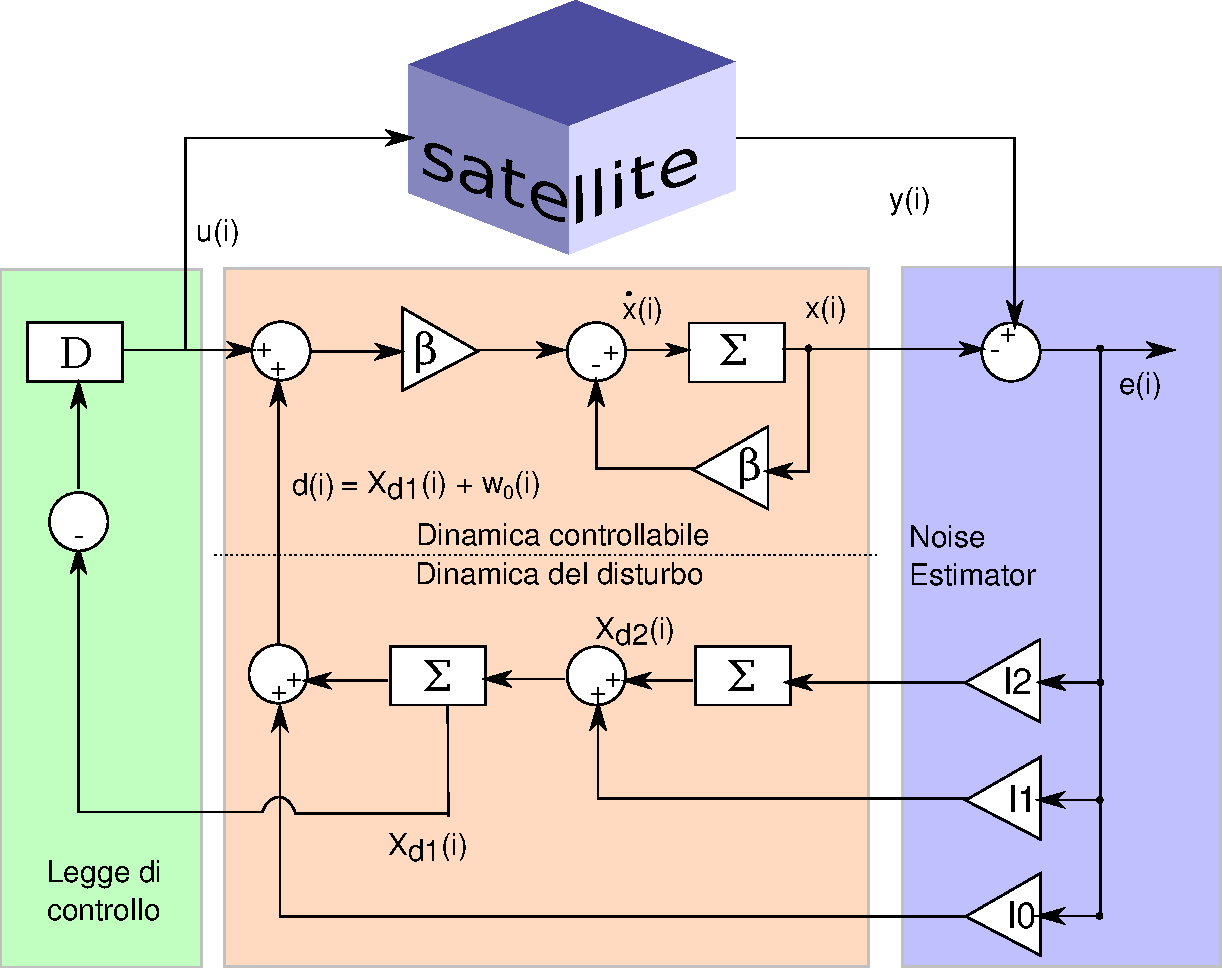
\includegraphics[width=\textwidth]{control/orbit_control/images/block-diagram.pdf}
\caption{Architettura del controllo}
\label{fig:orbit_control}
\end{figure}

\subsection{Equazioni e parametri del controllo}
In questa sottosezione ci occuperemo di descrivere nel dettaglio le equazioni
facenti capo a ciascun blocco funzionale precedentemente descritto:
%###
\paragraph{ Generatore dei riferimenti - Guidance:}
La funzione di questo blocco è quella di ricostruire il quaternione di
riferimento associato al riferimento LORF (Espresso nel sistema di riferimento
J2000) a partire dalle misure ricavate dall'unità GPS ($y_r$ posizione, $y_v$
velocità), richichiamando la definizione del LORF segue che:
\begin{equation}
	\mathfrak{R_0} = \{C,\bar{o}_1,\bar{o}_2,\bar{o}_3\}
\end{equation}

\begin{equation}
\bar{o}_1 = \frac{\vec{v}}{|\vec{v}|} \hspace{20pt}%
\bar{o}_2 = \frac{\vec{h}=\vec{r} \times \vec{v}}{|\vec{h}|} \hspace{20pt}%
\bar{o}_3 = \frac{\vec{e}=\bar{o}_1 \times \bar{o}_2}{|\vec{e}|}
\end{equation}

\begin{equation}
	\components{y_r}(t) = \components{r}(t) + \delta \components{r}(t)
\end{equation}

\begin{equation}
	\components{y_v}(t) = \components{v}(t) + \delta \components{v}(t)
\end{equation}

La matrice d'assetto LORF può essere ricavata come:
\begin{equation}
\underline{R_{0}^{i}}=
\begin{bmatrix}
	\frac{\components{y_v}}{|\components{y_v}|} &
	\frac{\components{y_h}=\components{y_r}	\times \components{y_v}}{|\components{y_h}|} &
	\frac{\components{y_e}=\components{y_v} \times (\components{y_r}\times\components{y_v})}{|\components{y_v}|}(t))
\end{bmatrix}
\end{equation}

La misura proventiente dal GPS é però affetta da errore per tanto definiamo la
matrice tenendo conto di una rotazione infinitesima definita
tramite gli angoli di eulero $\delta\components{\theta_0}$:
\begin{equation}
R_{0}^{i}=\underline{R_{0}^{i}}(I+\delta R_{0}^{i})
\end{equation}
\begin{equation}
\delta R_{0}^{i} = \delta\components{\theta_0} \times
\end{equation}
Un approssimazione degli angoli di eulero associati all'errore si ottiene
tramite la seguente relazione:

\begin{equation}
	\delta \boldsymbol{\theta_0}= \frac{1}{r}
	\begin{bmatrix}
	-\delta\vec{r}\cdot\vec{o}_2\\
	\delta\vec{r}\cdot\vec{o}_1-\frac{-\delta\vec{v}\cdot\vec{o}_3}{\omega_0}\\
	\frac{-\delta\vec{v}\cdot\vec{o}_2}{\omega_0}\\
	\end{bmatrix}
,\hspace{10pt} v\approx\omega_0 r 
\end{equation}

Calcoliamo adesso la varianza dell'errore di rotazione maggiorandola con una
quantità $\sigma^2_{0,max}$:
\begin{equation}
\xi[\delta\components{\theta_0}
\delta\components{\theta_0}^T]\le I \sigma^2_{0,max}
\end{equation}

Allocando la stessa varianza sia alla componente di posizione che di velocità
otteniamo che:

\begin{equation}
\sigma_r < \frac{(R_E + h)\cdot\sigma_{0,max}}{\sqrt{2}}
\end{equation}

\begin{equation}
\sigma_v < \frac{\omega_0\cdot r\cdot \sigma_{0,max}}{\sqrt{2}}
\end{equation}

tramite queste relazioni è possibile scegliere il sensore in grado di garantire
un errore angolare accettabile a partire dalle sue specifiche (varianza in
posizione e velocità).

Usando la conversione da matrice di assetto a quaternione è possibile calcolare
il quaternione di riferimento

\begin{equation}
	\underline{\components{\mathit{y_0}}}(t)=\underline{\components{\mathit{y_0}}}(\underline{R_{0}^{i}}(t))
\end{equation}

Svantaggio di questo approccio è l'impossibilità dell'ottenere il valore vero di
$\underline{R_{0}^{i}}$ poichè sarà sempre sporcato dall'errore di misura,
aggiungiamo quindi un predittore dello stato che ci permetta di filtrare questi
errori e che ci faccia guadagnare contemporaneamente anche la possibilità di
predirre il vettore accelerazione angolare orbitale
$\components{\underline{\dot{\omega}}}$ e velocità angolare orbitale
$\components{\underline{\omega}}$.
Definito l'incremento angolare come:
\begin{equation}
\components{\underline{\omega}^*} =\components{\underline{\omega}} \cdot T 
\end{equation}
dove $T$ è l'unità di tempo è possibile scrivere l'equazione di stato del quaternione:
\begin{IEEEeqnarray}{rCl}
\comp{\rif{\quat{q}}}(i+1)&=&c(i) \comp{\rif{\quat{q}}}(i) + \frac{1}{2} s(i)
\comp{\rif{\quat{q}}}(i) \otimes
\begin{bmatrix}
	0 \\
	\components{\underline{\omega}^*}
\end{bmatrix}, \hspace{20pt} \comp{\rif{\quat{q}}}(0)=\comp{\rif{\quat{q}}}_0 \\
c(i)&=&cos(\frac{|\comp{\underline{\omega}^*}(i)|}{2})\nonumber\\
s(i)&=&sin(\frac{|\comp{\underline{\omega}^*}(i)|}{2})
\frac{2}{|\comp{\underline{\omega}^*}(i)|}\nonumber
\end{IEEEeqnarray}
se $|\comp{\underline{\omega}^*}(i)|\ll 1$ allora $c(i) \approx s(i) \approx 1$
\begin{equation}
\comp{\rif{\quat{q}}}(i+1) =\comp{\rif{\quat{q}}}(i) + \frac{1}{2} 
\comp{\rif{\quat{q}}}(i) \otimes
\begin{bmatrix}
	0 \\
	\components{\underline{\omega}^*}
\end{bmatrix}, \hspace{20pt} \comp{\rif{\quat{q}}}(0)=\comp{\rif{\quat{q}}}_0 \\
\end{equation}
Consideriamo l'incremento angolare come la media all'interno dell'intervallo di
tempo \[\begin{bmatrix}iT, & (i+1) T \end{bmatrix}\].

All'interno di un architettura basata su predittore dello stato la velocità
angolare e l'accelerazione angolare devono diventare variabili di stato,
otteniamo quest'obiettivo tramite un modello stocastico aggiornato da un noise
estimator come effettuato precedentemente per il controllo orbitale:
\begin{equation}
	\begin{bmatrix}
		\comp{\rif{\omega}}^* \\
		\comp{\rif{a}}_q \\
		\comp{\rif{s}_q}
	\end{bmatrix}(i+1)
	=
	\begin{bmatrix}
		I & I & 0 \\
		0 & I & 0 \\
		0 & 0 & I \\
	\end{bmatrix}
	\begin{bmatrix}\comp{\rif{\omega}}^* \\ \comp{\rif{a}}_q \\
	\comp{\rif{s}_q}
	\end{bmatrix}(i)
	+		
	\begin{bmatrix}
		\comp{\rif{w}_\omega}\\
		\comp{\rif{w}_a}\\
		\comp{\rif{w}_s}\\	
	\end{bmatrix}(i)
	,\hspace{20pt}
	\begin{bmatrix}
		\comp{\rif{\omega}}^* \\
		\comp{\rif{a}}_q \\
		\comp{\rif{s}_q}
	\end{bmatrix}(0)
	=
	\begin{bmatrix}
		\comp{\rif{\omega}}^*_0 \\
		0 \\
		0 \\
	\end{bmatrix}
	\label{eq:attitude_state}
\end{equation}
dove $\comp{\rif{\omega}}^*_0$ è la velocità angolare orbitale nominale, e il
vettore
$\begin{bmatrix}\comp{\rif{w}_\omega}&\comp{\rif{w}_a}&\comp{\rif{w}_s}\end{bmatrix}^t$
un vettore di rumori bianchi stimati a partire dall'errore di modello:
\begin{equation}
\delta \rif{\comp{\quat{q}}}=\rif{\comp{\quat{q}}}^{-1} \otimes
\rif{\comp{\quat{y_0}}}
\label{eq:reference_model_error}
\end{equation}
facendo l'assunzione che l'errore di modello sia mantenuto piccolo dal
predittore dello stato possiamo approssimare l'eq
\ref{eq:reference_model_error}: tramite gli angoli di eulero
$\delta\rif{\comp{\theta}}$
\begin{equation}
	\delta \rif{\comp{\quat{q}}}
	=
	\begin{bmatrix}
		1 \\
		- - -\\
		\dfrac{\delta \rif{\comp{{\theta}}}}{2}
	\end{bmatrix}
\end{equation}
possiamo quindi per errori vicini allo zero scrivere una forma linearizzata
dell'equazione \ref{eq:attitude_state}
\begin{IEEEeqnarray}{rCl}
	\begin{bmatrix}
		\delta\rif{\theta}_{true,k}\\
		\delta\rif{\omega}^*_{true,k} \\
		\rif{a}_{q,k} \\
		\rif{s}_{q,k}
	\end{bmatrix}&(i+1)
	=&
	\begin{bmatrix}
		1 & 1 & 0 & 0 \\
		0 & 1 & 1 & 0 \\
		0 & 0 & 1 & 1 \\
		0 & 0 & 0 & 1 \\
		
	\end{bmatrix}
	\begin{bmatrix}
		\delta\rif{\theta}_{true,k}\\
		\delta\rif{\omega}^*_{true,k} \\
		\rif{a}_{q,k} \\
		\rif{s}_{q,k}
	\end{bmatrix}(i)
	+		
	\begin{bmatrix}
		0\\
		\rif{w}_\omega\\
		\rif{w}_a\\
		\rif{w}_s\\	
	\end{bmatrix}(i)
	,\\\nonumber
	\begin{bmatrix}
		\delta\rif{\theta}_{true,k}\\
		\delta\rif{\omega}^*_{true,k} \\
		\rif{a}_{q,k} \\
		\rif{s}_{q,k}
	\end{bmatrix}&(0)
	=&
	\begin{bmatrix}
		\comp{\rif{\theta}}_{true,0} \\
		0 \\
		0 \\
		0 \\
	\end{bmatrix},
	k=1,2,3
\end{IEEEeqnarray}
e definire l'errore di modello come
\begin{equation}
	\delta \theta_y (i) = 
	\begin{bmatrix}1 & 0 & 0 & 0\end{bmatrix}
	\begin{bmatrix}
			\delta\rif{\theta}_{true,k}\\
			\delta\rif{\omega}^*_{true,k} \\
			\rif{a}_{q,k} \\
			\rif{s}_{q,k}
	\end{bmatrix}(i) + 
	\delta\rif{\theta}(i)
\end{equation}
dove $\delta\rif{\theta}(i)$ è l'errore di misura, osserviamo come a parte un
fattore di scala 0.5 lo stesso ragionamento vale per il sistema non
linearizzato.
\'{E} possibile progettare adesso un noise estimator:
\begin{equation}
	\begin{bmatrix}
		\rif{w}_\omega\\
		\rif{w}_a\\
		\rif{w}_s\\	
	\end{bmatrix}
=
	\begin{bmatrix}
		\rif{l}_\omega\\
		\rif{l}_a\\
		\rif{l}_s\\	
	\end{bmatrix}
\delta\rif{\theta}(i)
\end{equation}
Si dimostra però che per qualunque scelta del vettore dei guadagni non si può
stabilizzare il predittore dello stato, si introduce quindi un quarto rumore
ottenuto ritardando l'uscita con una dinamica del primo ordine (introducendo
quindi una quinta variabile di stato) per arrivare all'equazione di stato finale
del predittore:

\begin{IEEEeqnarray}{rCl}
	\begin{bmatrix}
		\delta\rif{\theta}_{true,k}\\
		\delta\rif{\omega}^*_{true,k} \\
		\rif{a}_{q,k} \\
		\rif{s}_{q,k} \\
		\delta \rif{p}_k
	\end{bmatrix}&(i+1)
	=&
	\begin{bmatrix}
		1 & 1 & 0 & 0 & 0 \\
		-\rif{l}_{\omega} & 1 & 1 & 0 & \rif{m}_{\omega} \\
		-\rif{l}_{a} & 0 & 1 & 1 & \rif{m}_{a}\\
		-\rif{l}_{s} & 0 & 0 & 1 & \rif{m}_{s}\\
		-1 & 0 & 0 & 1 & 1 - \rif{\beta}\\
		
	\end{bmatrix}
	\begin{bmatrix}
		\delta\rif{\theta}_{true,k}\\
		\delta\rif{\omega}^*_{true,k} \\
		\rif{a}_{q,k} \\
		\rif{s}_{q,k} \\
		\delta \rif{p}_k
	\end{bmatrix}(i)
	+		
	\begin{bmatrix}
		0\\
		\rif{l}_\omega\\
		\rif{l}_a\\
		\rif{l}_s\\	
		1
	\end{bmatrix}\delta\theta_y(i)
	,\\\nonumber
	\begin{bmatrix}
		\delta\rif{\theta}_{true,k}\\
		\delta\rif{\omega}^*_{true,k} \\
		\rif{a}_{q,k} \\
		\rif{s}_{q,k} \\
		\delta \rif{p}_k
	\end{bmatrix}&(0)
	=&
	\begin{bmatrix}
		\comp{\rif{\theta}}_{true,0} \\
		0 \\
		0 \\
		0 \\
		0
	\end{bmatrix},
	k=1,2,3
\end{IEEEeqnarray}
Abbiamo qui 7 guadagni da poter tarare per avere una schedulazione degli
autovalori tale da stabilizzare il predittore
%###

\subsection{Simulazione e grafici}
Le simulazioni sono state ottenute abilitando nel simulatore le componenti
corrispondenti alle seguenti flags:
\begin{lstlisting}[language=matlab,breaklines=true]
GravityTypeFlag=1;		%(1=J2 Gravity Model/=0 Spherical)
GravityGradientTorqueFlag=1;	%1=Gravity Gradient Torque ON/0=OFF 
DragForceDisturbancesFlag=1;	%0=Drag Force Disturbance OFF/1=OFF
DragTorquesDisturbancesFlag=1;	%0=Drag Torque Disturbance OFF/1=ON
DragFreeControlFlag=1;		%0=Drag Free Control OFF/1=ON
AttitudeControlFlag=1;		%0=Attitude Control OFF/1=ON
\end{lstlisting}

\begin{SCfigure}[0.7][ht]
	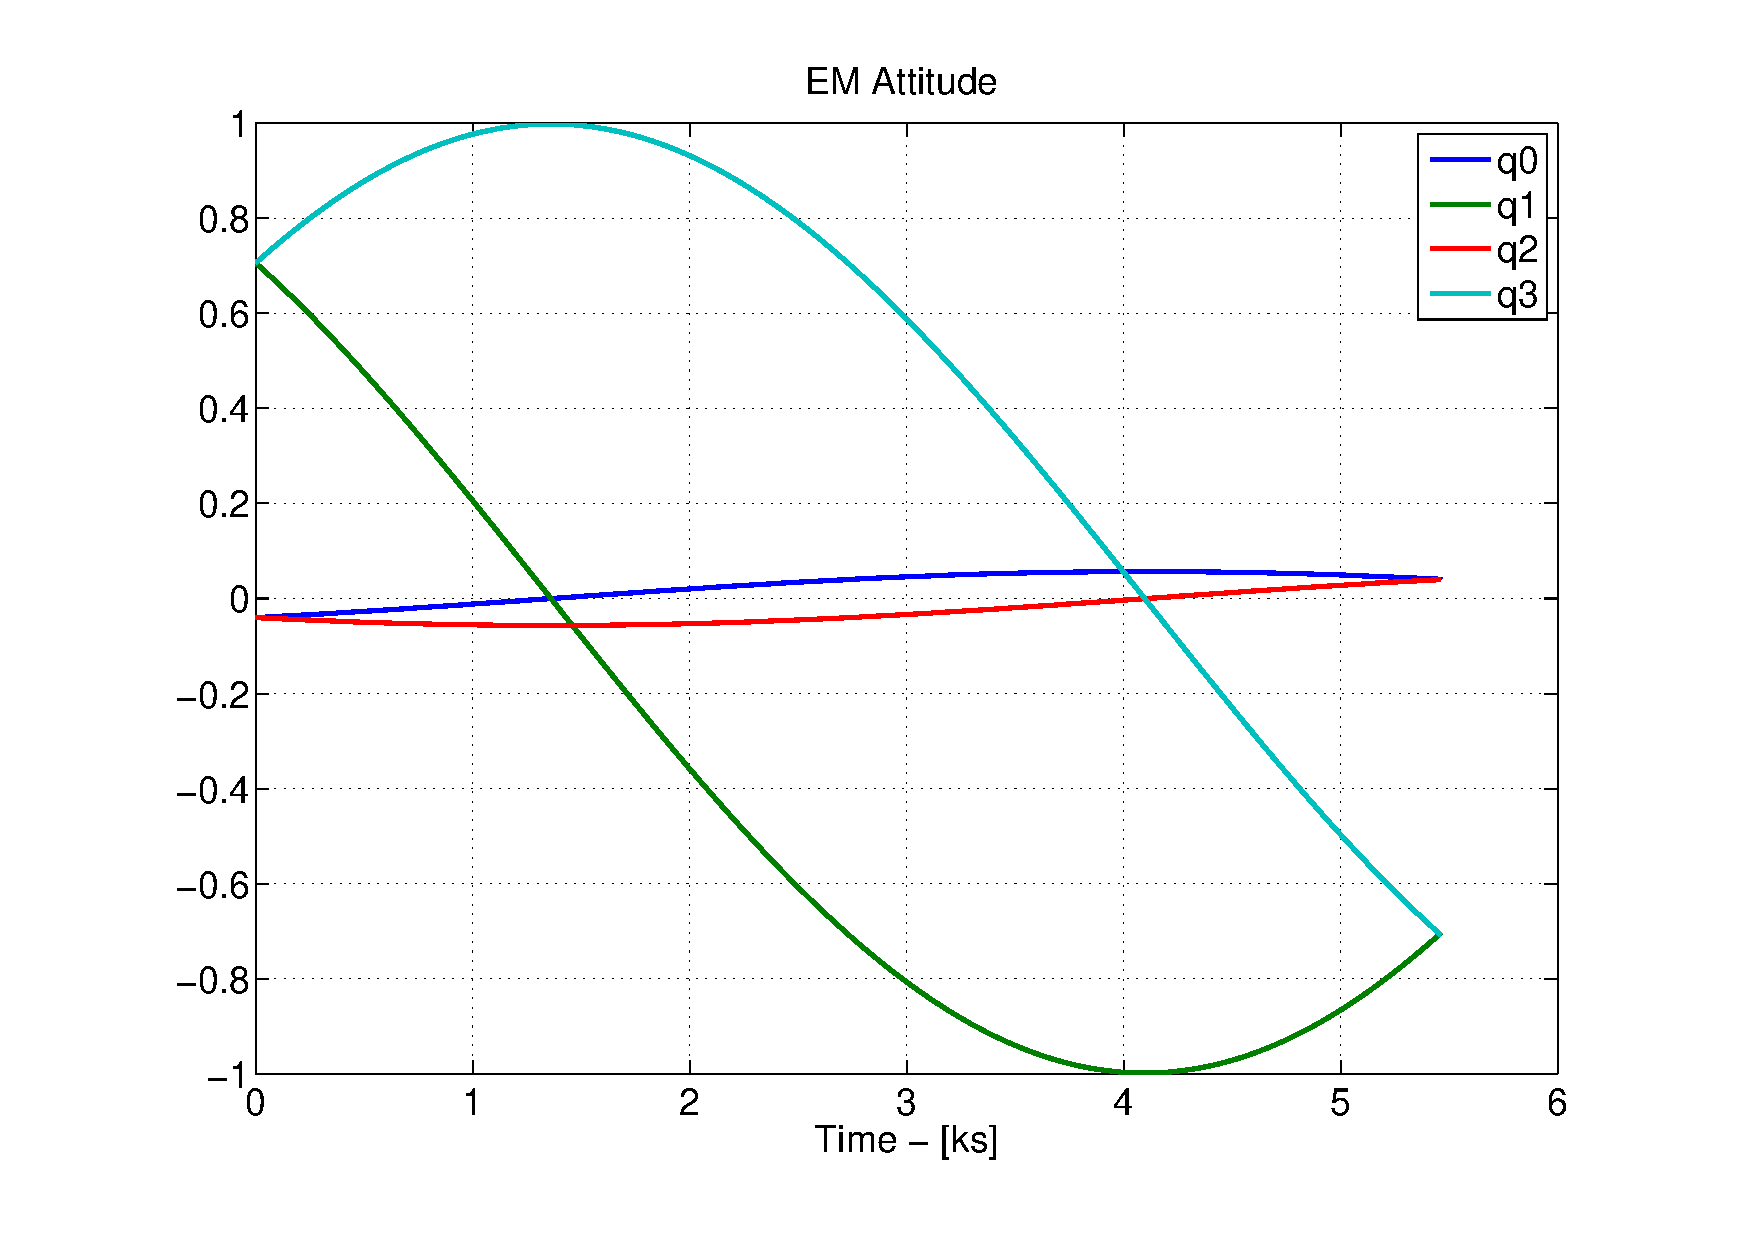
\includegraphics[width=.6\textwidth]{control/attitude_control/images/EmbeddedModelAttitude.pdf}
	\caption{\emph{Quaternione di assetto} --- Quaternione assetto stimato
	dall'embedded model a partire dallo star tracker}
	\label{fig:drag-acceleration}
\end{SCfigure}

\begin{SCfigure}[0.7][ht]
	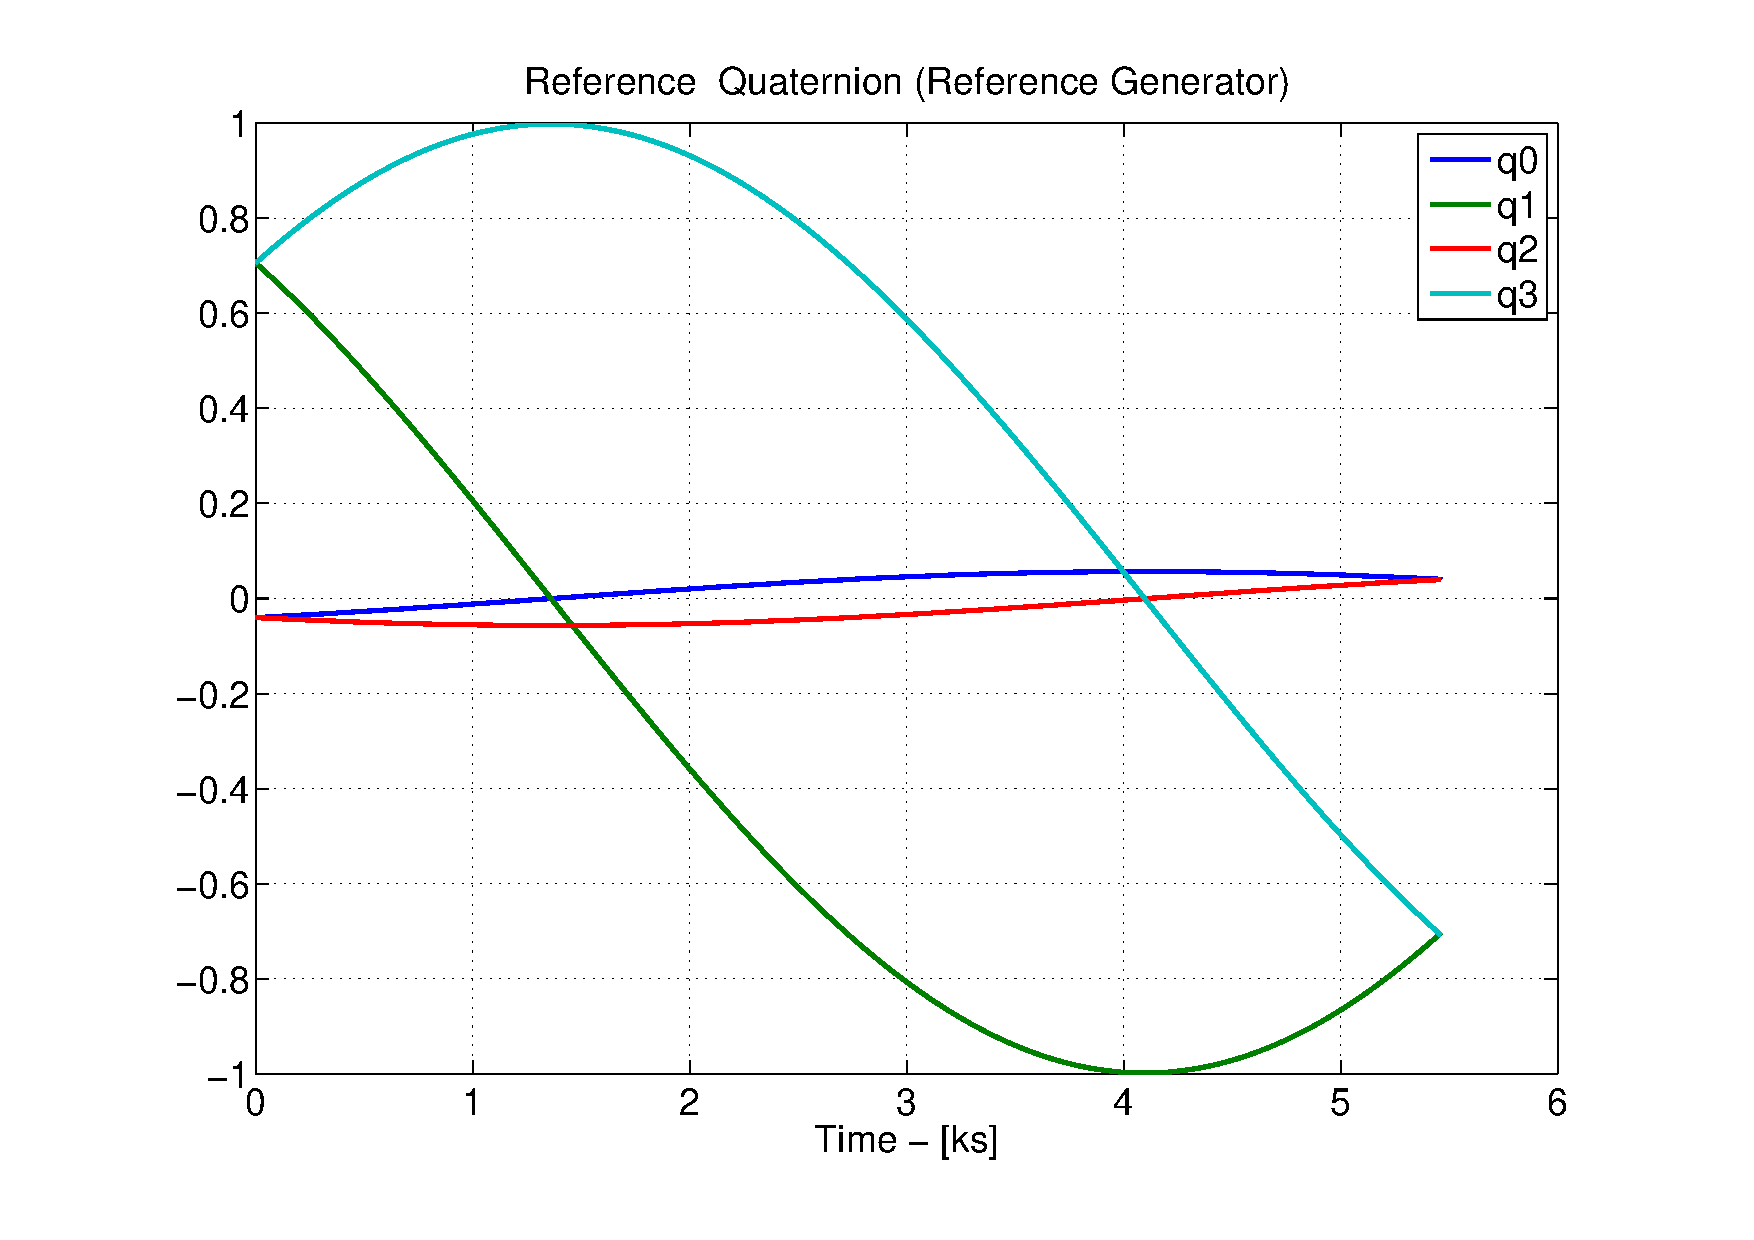
\includegraphics[width=.6\textwidth]{control/attitude_control/images/ReferenceQuaternion.pdf}
	\caption{\emph{Quaternione di riferimento} --- Quaternione rappresentante il
	riferimento LORF nel sistema di riferimento inerziale, deve essere inseguito
	dal controllo}
	\label{fig:drag-acceleration}
\end{SCfigure}

\begin{SCfigure}[0.7][ht]
	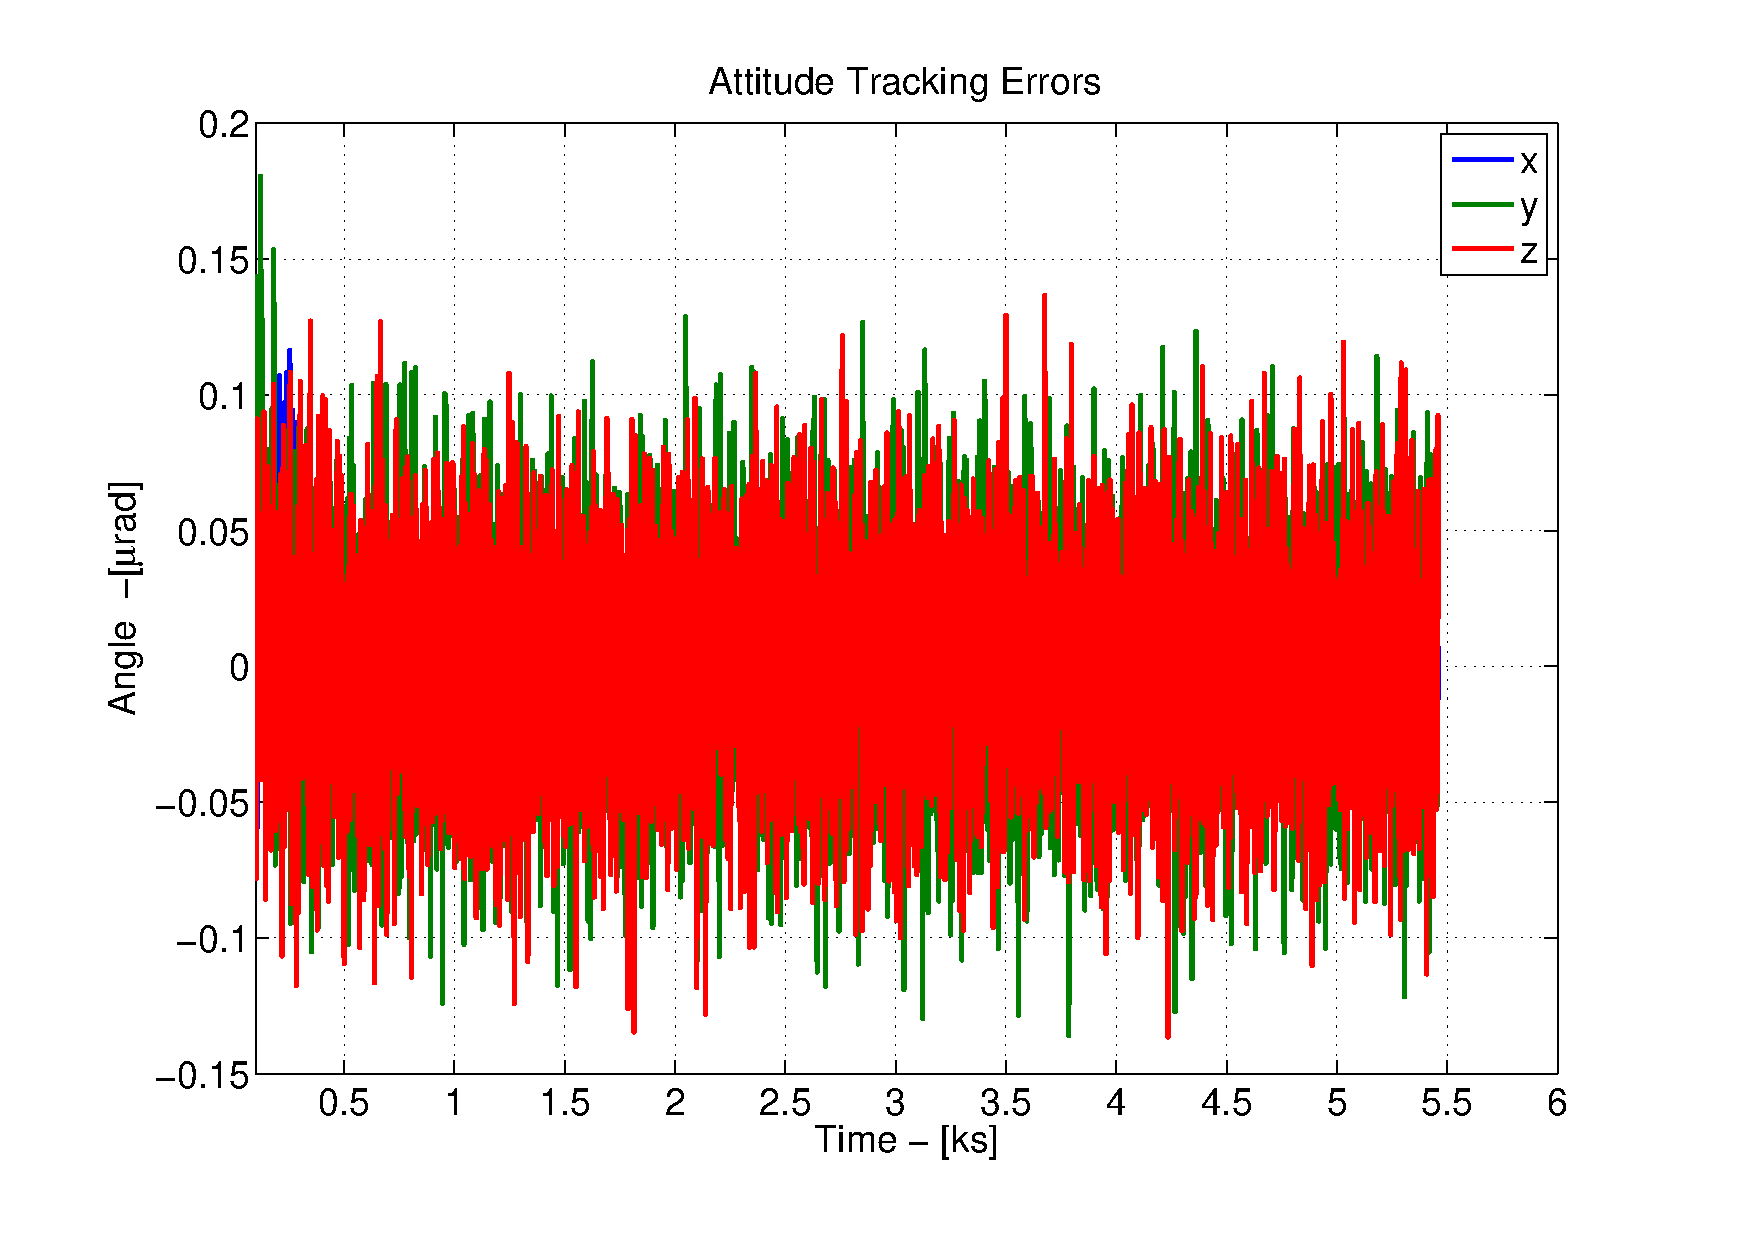
\includegraphics[width=.6\textwidth]{control/attitude_control/images/TrackingError.pdf}
	\caption{\emph{Errore di inseguimento} --- L'errore si mantiene nei requisiti
	di precisione richiesti}
	\label{fig:drag-acceleration}
\end{SCfigure}
%###